\documentclass{beamer}



\usepackage[french]{babel}
\frenchbsetup{StandardLists=true} 

\usepackage[utf8]{inputenc}
\usepackage{palatino}
\usepackage[T1]{fontenc}

\usepackage{beamerthemeshadow}
\usepackage{listings}
\lstset{
language=Java,
basicstyle=\ttfamily\small, %
identifierstyle=\color{black}, %
keywordstyle=\color{blue}, %
stringstyle=\color{blue}, %
commentstyle=\it\color{green}, %
}


%-------------------------------------------------------------

%\vspace{-1cm}



%-------------------------------------------------------------
\begin{document}
  %\addtocounter{framenumber}{-1} 

  \begin{frame}
    \begin{figure}[H]
      \centering
      
\includegraphics[scale=1]{image/logo.jpg} 
      \label{fig:logo}
    \end{figure}
   
  \end{frame}

   \section{JADE}
  \begin{frame}
    JADE (Java Agent DEvelopment Framework) est un framework Java (multi-platform) pour le développement multi-agent.
    
    Il contient :
    \begin{itemize}
      \item Un environnement de travail.
      \item Une bibliothèque contenant différents outils.
      \item Des outils Graphiques.
    \end{itemize}
  \end{frame}
  
  \begin{frame}
    Jade possède trois modules principaux (nécessaire aux normes FIPA).
    
    \begin{description}
      \item[DF "Director Facilitor"] fournit un service de "pages jaunes" à la plate-forme.
      \item[ACC "Agent Communication Channel"] gère la communication entre les agents.
      \item[AMS "Agent Management System"] supervise l'enregistrement des agents, leur authentification, leur accès et l'utilisation du système.
    \end{description}
  \end{frame}
  
  \begin{frame}
   Par ailleurs, la plate-forme possède une architecture très précise permettant la construction dite "normalisés" d’agents. 
   Pour cela, elle se décompose en plusieurs classes:
   \begin{figure}[H]
      \centering
      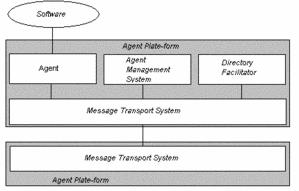
\includegraphics[scale=0.5]{image/fipa.jpg} 
      \label{fig:échiquierDebut}
  \end{figure}
  \end{frame}
  
\end{document}